\section{External Validation}
\label{sec:external}

We ask whether the WAL tail hurts questions without updates, whether the erasure finding holds for a production memory library, and whether epoch ordering helps on a second, independently built conflict dataset.

\subsection{Non-update questions}
\label{sec:regression}

On \nm{datasets/regression60/All} LongMemEval-S questions disjoint from the held-out set (multi-session and single-session user, assistant and preference questions; Table~\ref{tab:regression60} in Appendix~\ref{app:tables}), DeltaWAL-Versioned at lag 0 scores at least as well as B1 for every reader (\nm{tab3/gemma4/deltawal_versioned/lag0/All}\% vs.\ \nm{tab3/gemma4/B1_sync/lag0/All}\% for gemma4, \nm{tab3/gpt-6-luna/deltawal_versioned/lag0/All}\% vs.\ \nm{tab3/gpt-6-luna/B1_sync/lag0/All}\% for gpt-6-luna, \nm{tab3/glm-5.3/deltawal_versioned/lag0/All}\% vs.\ \nm{tab3/glm-5.3/B1_sync/lag0/All}\% for glm-5.3). The intervals overlap, so we read this as no regression, not as an improvement. Single-session-assistant questions expose extraction loss: the extractor sees assistant turns truncated to \nm{frozen_config/assistant_trunc_chars_extract} characters, so B1 answers \nm{tab3/gemma4/B1_sync/lag0/single-session-assistant}\% of them for every reader. At lag 1 the evidence session is still in the WAL and DeltaWAL-Versioned answers \nm{tab3/gemma4/deltawal_versioned/lag1/single-session-assistant}\%, \nm{tab3/gpt-6-luna/deltawal_versioned/lag1/single-session-assistant}\% and \nm{tab3/glm-5.3/deltawal_versioned/lag1/single-session-assistant}\% from the raw turns. This is not a lasting gain: once the session commits, the detail is gone again.

\subsection{\memzero{} OSS with in-place updates}
\label{sec:mem0}

% generated by scripts/build_paper_assets.py -- do not edit by hand
\begin{table*}[t]
\centering
\small
\setlength{\tabcolsep}{4pt}
\caption{Mem0 OSS 1.0.11 (classic ADD/UPDATE/DELETE write path) on the 60 held-out knowledge-update questions. Mem0 sync ingests every session; Mem0 async leaves the final (update) session in flight; Mem0 + DeltaWAL adds the epoch-tagged WAL and relevance gate ($\tau=0.35$) on top of the async store. The history hook renders, for every retrieved memory, its earlier versions from \texttt{Memory.history()} in epoch order (run on the KU-past questions only; $^\ast$stale rate over those questions). On the 13 KU-past questions Mem0 updated the older evidence memory in place in 11 and deleted it in 0.}
\label{tab:mem0}
\begin{tabular}{lrcccc}
\toprule
System & Lag & \begin{tabular}[b]{@{}c@{}}KU\\($n$=60)\end{tabular} & \begin{tabular}[b]{@{}c@{}}KU-past\\($n$=13)\end{tabular} & \begin{tabular}[b]{@{}c@{}}KU-current\\($n$=47)\end{tabular} & \begin{tabular}[b]{@{}c@{}}Stale\\(\%)\end{tabular} \\
\midrule
\multicolumn{6}{l}{\textit{Reader: gemma4 (12B, local)}} \\
Mem0 sync & 0 & 76.7\,{\scriptsize[65, 87]} & 46.1\,{\scriptsize[23, 69]} & 85.1\,{\scriptsize[74, 94]} & 6.7 \\
Mem0 async & 1 & 10.0\,{\scriptsize[3, 18]} & 46.1\,{\scriptsize[23, 77]} & 0.0\,{\scriptsize[0, 0]} & 66.7 \\
Mem0 + DeltaWAL & 1 & 91.7\,{\scriptsize[83, 98]} & 92.3\,{\scriptsize[77, 100]} & 91.5\,{\scriptsize[83, 98]} & 6.7 \\
Mem0 sync + history hook & 0 & -- & 100.0\,{\scriptsize[100, 100]} & -- & 0.0$^\ast$ \\
\midrule
\multicolumn{6}{l}{\textit{Reader: gpt-6-luna (cloud)}} \\
Mem0 sync & 0 & 76.7\,{\scriptsize[65, 87]} & 53.9\,{\scriptsize[31, 77]} & 83.0\,{\scriptsize[72, 94]} & 6.7 \\
Mem0 async & 1 & 11.7\,{\scriptsize[5, 20]} & 53.9\,{\scriptsize[31, 85]} & 0.0\,{\scriptsize[0, 0]} & 63.3 \\
Mem0 + DeltaWAL & 1 & 96.7\,{\scriptsize[92, 100]} & 100.0\,{\scriptsize[100, 100]} & 95.7\,{\scriptsize[89, 100]} & 1.7 \\
Mem0 sync + history hook & 0 & -- & 100.0\,{\scriptsize[100, 100]} & -- & 0.0$^\ast$ \\
\midrule
\multicolumn{6}{l}{\textit{Reader: glm-5.3 (frontier, cloud)}} \\
Mem0 sync & 0 & 76.7\,{\scriptsize[65, 87]} & 46.1\,{\scriptsize[23, 69]} & 85.1\,{\scriptsize[74, 94]} & 5.0 \\
Mem0 + DeltaWAL & 1 & 96.7\,{\scriptsize[92, 100]} & 100.0\,{\scriptsize[100, 100]} & 95.7\,{\scriptsize[89, 100]} & 0.0 \\
Mem0 sync + history hook & 0 & -- & 100.0\,{\scriptsize[100, 100]} & -- & 0.0$^\ast$ \\
\bottomrule
\end{tabular}
\par\medskip
\begin{tabular}{lrrr}
\toprule
Mem0 history events (60 questions) & ADD & UPDATE & DELETE \\
\midrule
sessions $1..T{-}1$ (async view) & 6913 & 152 & 3 \\
sessions $1..T$ (sync view) & 7125 & 265 & 5 \\
KU-past subset, sessions $1..T$ ($n$=13) & 1539 & 52 & 0 \\
\bottomrule
\end{tabular}
\end{table*}


We ran \memzero{} OSS~\citep{chhikara2025mem0}, pinned to version \nm{frozen_config/mem0_version}, on the \nm{datasets/mem0_ku60/n} held-out KU questions. Each \texttt{add()} extracts facts with one LLM call and then decides, against similar existing memories, whether to ADD, UPDATE, DELETE or do nothing; UPDATE rewrites a memory in place, and the old text survives only in a history table exposed by \texttt{Memory.history()}, not by search. Mem0 2.x has an add-only write path that cannot exercise UPDATE, so we did not use it. Each question's history was ingested once (internal LLM: gpt-6-luna) and shared across readers. \emph{\memzero{} sync} reads after all sessions are ingested, \emph{\memzero{} async} with the update session in flight, and \emph{\memzero{} + DeltaWAL} adds the gated WAL tail with epoch tags and the precedence instruction. The \emph{history hook} is a read-only ablation on \memzero{} sync that renders each retrieved memory's earlier versions from \texttt{Memory.history()} in epoch order.

\memzero{} sync loses KU-past questions as our mutable store does: \nm{tab4/gemma4/Mem0_sync/lag0/KU_past}\%, \nm{tab4/gpt-6-luna/Mem0_sync/lag0/KU_past}\% and \nm{tab4/glm-5.3/Mem0_sync/lag0/KU_past}\% (gemma4, gpt-6-luna, glm-5.3), against \nm{tab4/gemma4/Mem0_sync/lag0/KU_current}\%--\nm{tab4/gpt-6-luna/Mem0_sync/lag0/KU_current}\% on KU-current (Table~\ref{tab:mem0}). On \nm{tab4/ku_past_flags/old_value_updated_in_place} of the \nm{datasets/mem0_ku60/KU_past} KU-past questions it updated the older evidence memory in place. UPDATE events are rare overall (\nm{tab4/history_events/sessions_1..T_sync_view/UPDATE} against \nm{tab4/history_events/sessions_1..T_sync_view/ADD} ADD events) but fall on exactly the facts these questions ask about. \memzero{} async goes stale like B2 (KU-current \nm{tab4/gemma4/Mem0_async/lag1/KU_current}\% for both readers run). The DeltaWAL wrapper adds no state to \memzero{} and raises KU accuracy to \nm{tab4/gemma4/Mem0_deltawal/lag1/KU}\%--\nm{tab4/glm-5.3/Mem0_deltawal/lag1/KU}\%; its KU-past result has the same cause as in Section~\ref{sec:hist-write}, since at lag 1 \memzero{} has not yet applied the update. The history hook covers the committed state: it raises KU-past accuracy of \memzero{} sync to \nm{tab4/gemma4/Mem0_sync_history/lag0/KU_past}\% for all three readers. The old value was never lost; it sat in an audit table that the read path does not show, and on \nm{tab4/ku_past_flags/gold_old_value_only_in_history} questions it was the only remaining copy. The degenerate intervals reflect sample size, not certainty.

\subsection{MemConflict}
\label{sec:memconflict}

MemConflict~\citep{tao2026memconflict} generates synthetic multi-session dialogues in two stages, a session synopsis and then the dialogue, and plants three conflict types. In a \emph{dynamic} conflict a value changes and the newer one is correct; in a \emph{static} conflict a later session contradicts a stable fact and the later statement is designated false; in a \emph{conditional} conflict the applicable value depends on context. We drew \nm{datasets/memconflict/All} questions, \nm{datasets/memconflict/Dynamic} per type, and audited each blind to model outputs with two LLM raters (Appendix~\ref{app:memconflict}). \nm{memconflict_audit90/clean} and \nm{memconflict_audit90_r2/clean} questions are clean for the two raters, below our pre-set gate of \nm{memconflict_audit90/gate_pct}\%; the raters agree on \nm{memconflict_audit90_r2/agreement_binary_pct}\% of questions (Cohen's $\kappa=\nm{memconflict_audit90_r2/kappa_binary}$). Quality differs by type: \nm{tab8/dynamic/evaluated/clean_both} of \nm{tab8/dynamic/evaluated/n} dynamic questions are clean for both raters, but only \nm{tab8/static/evaluated/clean_both} of \nm{tab8/static/evaluated/n} static ones, mostly because the later statement does not logically contradict the earlier one (a Bachelor's degree does not refute a Master's). We therefore use the dynamic type as a replication and treat the static type as exploratory. Results below use the \nm{memconflict_audit90_r2/both_clean} questions both raters call clean; Appendix~\ref{app:tables} has full-set tables.

\paragraph{Dynamic conflicts replicate the staleness result.}
Pooled over three readers, DeltaWAL-Versioned answers \nm{tab7/pooled/deltawal_versioned/lag0/dynamic}\% of the clean dynamic questions at lag 0 and \nm{tab7/pooled/deltawal_versioned/lag1/dynamic}\% at lag 1, B1 \nm{tab7/pooled/B1_sync/lag0/dynamic}\%, and B2 and B3 at lag 1 \nm{tab7/pooled/B2_async/lag1/dynamic}\% and \nm{tab7/pooled/B3_recency_matched_user/lag1/dynamic}\% (Figure~\ref{fig:external}b). The ordering matches LongMemEval-S; the DeltaWAL-Versioned and B1 intervals overlap.

\paragraph{Static conflicts (exploratory).}
Here epoch precedence is the wrong rule by construction. On the clean static questions DeltaWAL-Versioned at lag 0 answers with the later, false statement on \nm{tab7/pooled/deltawal_versioned/lag0/static_false_belief}\% (\nmci{tab7/pooled/deltawal_versioned/lag0/static_false_belief}) against \nm{tab7/pooled/B1_sync/lag0/static_false_belief}\% for B1, whose prompt has no precedence rule; the point estimate is higher for every reader and in every audit subset, but the set is small (\nm{tab8/static/evaluated/clean_both} questions) and the intervals overlap. B2 and B3 rarely believe the false statement only because it sits in the in-flight session, which B2 never sees and B3 sees as undated raw text. We read this as a boundary of the design rather than a measured effect size: newer-wins precedence assumes that a later statement is more correct, and false corrections need a different policy, such as checking the source of a correction or confirming a change to a stable fact against the version history.

\begin{figure*}[t]
\centering
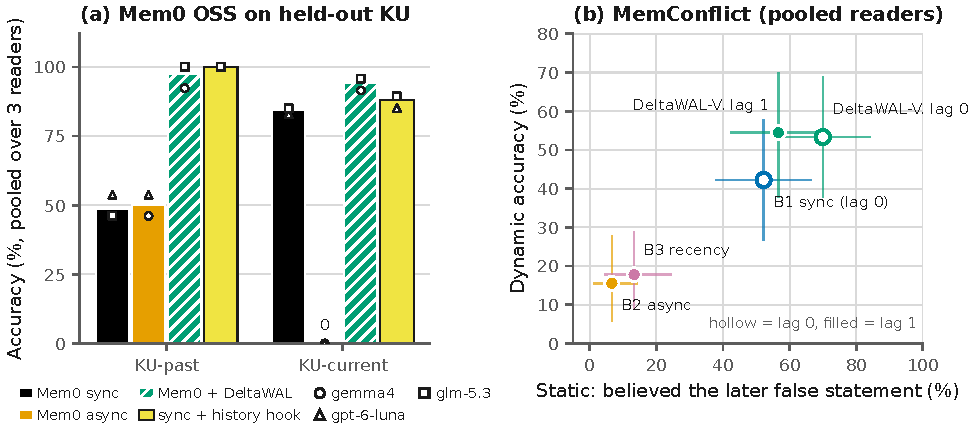
\includegraphics[width=\textwidth]{figures/fig4_external.pdf}
\caption{External validation, pooled over readers. (a) \memzero{} OSS on the \nm{datasets/mem0_ku60/n} held-out KU questions: \memzero{} sync loses KU-past (\nm{fig4/mem0_pooled/Mem0_sync/KU-past}\%) because UPDATE overwrites in place; \memzero{} async loses KU-current (\nm{fig4/mem0_pooled/Mem0_async/KU-current}\%); the DeltaWAL wrapper at lag 1 scores \nm{fig4/mem0_pooled/Mem0_deltawal/KU-past}\% and \nm{fig4/mem0_pooled/Mem0_deltawal/KU-current}\%; the read-only history hook recovers KU-past (\nm{fig4/mem0_pooled/Mem0_sync_history/KU-past}\%). Markers show individual readers; \memzero{} async was not run with glm-5.3. (b) MemConflict, all \nm{datasets/memconflict/All} questions: dynamic accuracy against the rate of believing the later, false statement on static questions (exploratory); hollow markers lag 0, filled lag 1, bars \nm{stats/ci_level_pct}\% intervals. The clean-subset values are in the text and Table~\ref{tab:memconflict_clean}.}
\label{fig:external}
\end{figure*}
